%% mylatex/ieicej:3.4a のサンプル（論文）
%% コンパイル: docker run --rm -v "$PWD":/work mylatex/ieicej:3.4a
\documentclass[paper]{style/ieicej}
\usepackage[dvipdfmx]{graphicx,xcolor}
\usepackage[fleqn]{amsmath}
\usepackage{newtxtext}% 英数字フォントの設定を変更しないでください
\usepackage[varg]{newtxmath}% 英数字フォントの設定を変更しないでください

\setcounter{page}{1}

\field{}
\jtitle{Dockerによる\LaTeX{}コンパイル環境の構築}
\etitle{Building a \LaTeX{} Compilation Environment with Docker}
\authorlist{%
 \authorentry{電子 太郎}{Taro DENSHI}{kobe}\MembershipNumber{}
}
\affiliate[kobe]{神戸大学}{Kobe University}
\jalcdoi{???????????}% ← このままにしておいてください

\begin{document}
\begin{abstract}
本稿では，学会スタイルごとにDockerイメージを作成し，
\LaTeX{}原稿をコンテナ内でコンパイルする方法を示す．
\end{abstract}
\begin{keyword}
Docker，\LaTeX{}，コンパイル環境
\end{keyword}
\begin{eabstract}
This paper shows how to compile \LaTeX{} manuscripts in a container
built for each journal style.
\end{eabstract}
\begin{ekeyword}
Docker, \LaTeX{}, build environment
\end{ekeyword}
\maketitle

\section{まえがき}
\label{sec:intro}

学会ごとに配布されるスタイルファイルは版によって挙動が異なるため，
執筆者ごとに環境を揃えることは容易ではない\cite{knuth1984}．
本稿では，スタイル一式を焼き込んだコンテナを用いてこの問題を解決する\cite{denshi2024}．
\ref{sec:method}章で手法を述べる．

コンパイル時間$T$は，パス数$n$と1パスあたりの時間$t_i$を用いて
\begin{equation}
  T = \sum_{i=1}^{n} t_i
  \label{eq:time}
\end{equation}
と表される．

\section{提案手法}
\label{sec:method}

図\ref{fig:pdf}にPDF形式の図，図\ref{fig:png}にPNG形式の図の例を示す．
式(\ref{eq:time})のパス数$n$はlatexmkが自動で決定する．

\begin{figure}[tb]
  \centering
  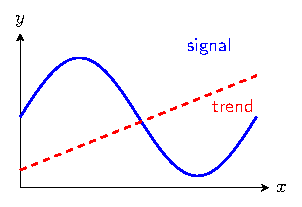
\includegraphics[width=0.9\columnwidth]{fig/sample.pdf}
  \caption{PDF形式の図}
  \label{fig:pdf}
\end{figure}

\begin{figure}[tb]
  \centering
  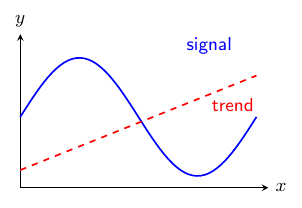
\includegraphics[width=0.6\columnwidth]{fig/sample-raster.png}
  \caption{PNG形式の図}
  \label{fig:png}
\end{figure}

\begin{table}[tb]
  \centering
  \caption{エンジンと出力形式}
  \label{tab:engine}
  \begin{tabular}{ll}
    \hline
    エンジン & 出力 \\
    \hline
    uplatex  & DVI $\rightarrow$ PDF (dvipdfmx) \\
    pdflatex & PDF \\
    \hline
  \end{tabular}
\end{table}

表\ref{tab:engine}に対応するエンジンを示す．


\ack
本サンプルの作成にあたり，ご協力いただいた皆様に感謝する．

\bibliographystyle{style/sieicej}
\bibliography{bib/refs}

\end{document}
